%!TEX root = ../dissertation.tex

\Chapter{Supplementary information for Chapter~\ref{sec:planning}}\label{app:planning}

\section{Deviations from pre-registration}\label{app:planning-deviations}
Here we document all deviations our pre-registered analysis plans.

For several experiments we recruited slightly more participants than originally intended as a result of participants completing the experiment after being flagged as incomplete by Prolific.

In Experiments 1 and 3, we pre-registered proportion tests for best-first search and the forward search bias. We switched to Wilcoxon tests over participants means as this test correctly respects the group structure of the experiment. The qualitative conclusions are the same with either approach. The original results were $z=72.1,\ p < .001$ for best-first search and $z=51.1,\ p < .001$ for expansion.

Similarly, in Experiments 1 and 4, we initially performed fixed effects logistic regressions, but decided that mixed-effects regressions were more principled. The qualitative conclusions are the same with either approach, although the coefficients are substantially larger with the mixed-effects regression. For Experiment 1, the fixed-effects regression coefficient for best path value is $\beta = 0.579$ (95\% CI [0.521, 0.637], $z = 19.6$, $p < .001$); for best vs. next, $\beta = 1.111$ (95\% CI [1.059, 1.163], $z = 41.9$, $p < .001$. This is compared to $\beta = 0.539$ and $\beta = 1.900$ in the optimal model. For Experiment 4, the fixed-effects regression coefficient for value on violation of forward search is $\beta = 0.579$, 95\% CI [0.465, 0.694], $z = 9.9$, $p < .001$.

In Experiment 1, we pre-registered that we would report the difference in likelihood between the optimal model and the best model without best vs. next. We ultimately decided that this comparison was not of special interest. The likelihood difference is $\dnll = 1911$ in favor of the optimal model.

For Experiment 2, we pre-registered that we would report the difference in likelihood between the best-fitting model and the next-best-fitting model. However, we later decided that the difference from the optimal model was a more useful comparison in the constant variance case, where the optimal model did not fit best. The best-fitting model in that case was the best-first model with best vs. next and depth limits. The next best model (excluding other best-first variants) was depth-first with satisficing, depth limits, and pruning ($\dnll = 885$).

\begin{figure*}[t!]
    \centering
    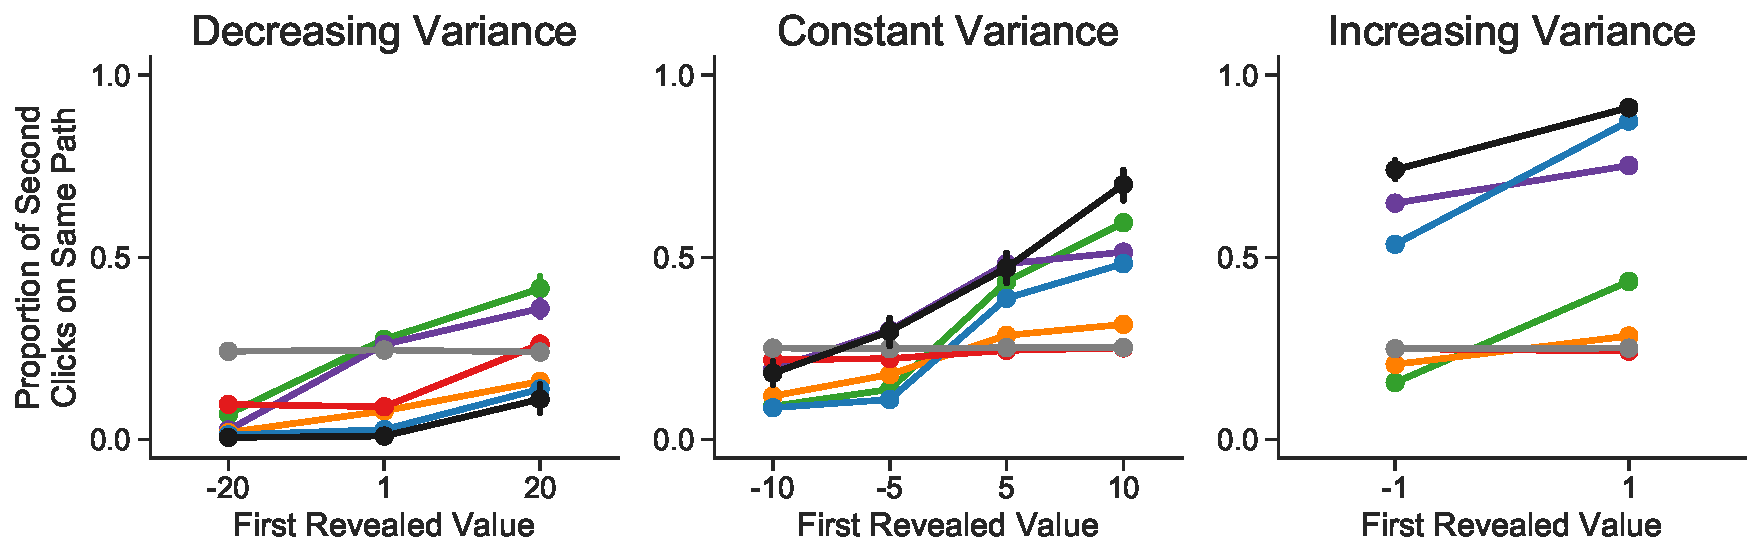
\includegraphics[width=\textwidth]{figs/planning/second_click_alt.pdf}
    \caption{\captiontitle{Alternative version of Figure~\ref{fig:planning-exp2}D}. Here, the predictions of all alternative models are genreated with the best-fitting set of heuristic mechanisms. As in Figure~\ref{fig:planning-exp2}D, points show means and error bars show bootstrapped 95\% confidence intervals, both computed across participants ($n=$108, 91, and 90 for the left, center, and right panels).
    }
    \label{fig:second_click_alt}
\end{figure*}

For main-text Figure~4D, we pre-registered that we would plot the predictions of the same models shown in main-text Figure~4D. However, as illustrated in Figure~\ref{fig:second_click_alt}, the pruning mechanism allows depth-first search to closely mimic best-first search on the second click (although not necessarily on later clicks, as the model comparison reveals). We ultimately decided that it was more important to convey the qualitative difference between the different search orders than to show how the heuristic mechanisms can improve the fit to data. For this reason, we switched to plotting the predictions of the best-, breadth-, and depth-first models without any heuristic mechanisms.

For Experiment 3, we neglected to mention that we would not consider pruning and depth limits in the model comparison. As stated in the main text, it is not clear how to generalize these mechanisms to the case where there is not a forward search constraint. Furthermore, the most obvious generalizations that effectively treat each node independently (rather than operating on branches of a decision tree) make computing the likelihood excessively computationally intensive due to the need to marginalize over all possible pruning decisions (see Methods). Importantly, the initial omission was simply an error in the preparation of the pre-registration document. We decided to omit these mechanisms long before running the experiment, when we discovered that we could not apply the existing implementation of pruning and depth limits to pilot data.

\section{Experiment 5: Interleaved planning and action}\label{app:planning-experiment5}


\begin{figure}[t!]
    \centering
    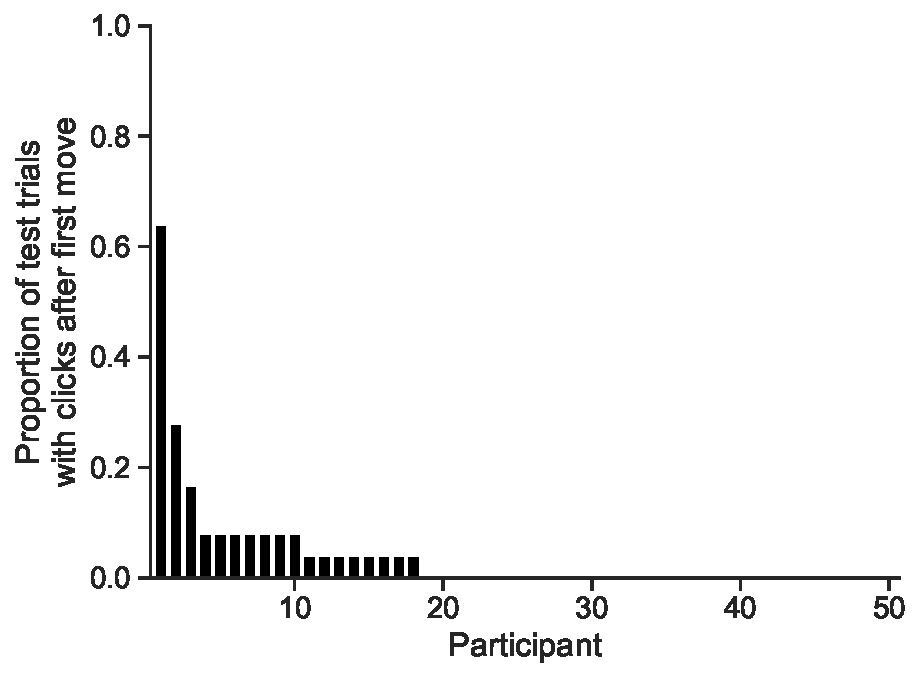
\includegraphics[width=0.7\textwidth]{figs/planning/interleaved.pdf}
    \caption{\captiontitle{Experiment 5 results.} The proportion of test trials in which each participant made at least one click after moving the spider.}
    \label{fig:exp5}
\end{figure}


In Experiments 1-3, we constrained participants to do all their planning (clicking) before taking their first action (moving the spider). We constrained the task in this way for two reasons: First, the optimal policy always does all its planning before taking any action; this is because moving cannot inform future planning but further planning could make one regret moves one has already made (in which case, one should have done that planning earlier). Second, allowing participants to violate this principle would require modifying the model to account for this possibility; this would complicate the implementation substantially. However, one could argue that by constraining participants to do all of their planning upfront, we are forcing them to follow the optimal strategy in this regard. It is thus important to know whether people would violate the principle if given the opportunity.

To address this question, we ran an experiment that was exactly like Experiment~1 except that we allowed participants to click at any time (even after moving). This was visually indicated by highlighting the clickable frontier nodes after each movement, with the frontier expanding to include states adjacent to the spider's new location. The results are illustrated in Figure~\ref{fig:exp5}. We found that participants very rarely chose to click after moving the spider. Although 36 out of 50 participants (72\%) revealed a reward after moving the spider on at least one practice trial (suggesting that they understood it was possible to do so), only 3 participants (6\%) clicked after moving on more than 2 out of the 25 test trials. Overall, participants clicked after moving on 3.9\% of test trials. This perhaps reflects a sensitivity to the informational asymmetry of moving and planning described above.


\section{Probability-based stopping rules}\label{app:planning-probstop}
In the main text, we considered two heuristic stopping rules based on the expected values of the best and second-best paths, satisficing and best vs. next. These stopping rules are truly heuristic, in the sense that they are very easy to compute. However, by reducing paths to their expected value, they potentially throw away useful information about the \emph{distribution} of possible values the path could take. Thus, we also considered more sophisticated variants of each stopping rule which are based on probabilities rather than expected values. These stopping rules involve extensive computation (concretely, marginalizing over joint distributions over possible path values) and are thus not truly ``heuristic''. However, they can potentially provide insight into which aspects of our partcipants' reasoning the heuristic models fail to capture.

\subsection{Model}
First, some notation. Let $V_i$ be a random variable describing the distribution of possible values path $i$ could have and let $b$ be the path with highest expected value (we address ties below). 

The probabilistic satisficing term is defined $\Pr(V_{b} \geq \alpha)$ where $V_{b}$ is a the true value of the best path and $\alpha$ is a threshold. If multiple paths have maximal expected value, we compute the term for all paths and use the maximum. We refer to this component of the stopping rule as ``prob better'' as it gives the probability that the best path is better than some value.

The probabilistic best vs. next term could be defined in several ways, the primary decision being whether to choose the competing value based on the current expected values or instead based on hypothetical true values. We chose the latter as it produces an intuitively appealing quantity: the probability that the path with best expected value in fact has maximal value. Thus, abusing the max operator slightly, we have $\Pr(V_{b} \geq \max_{i \neq b} V_i)$ where $\max_{i \neq b} V_i$ should be interpreted as a random variable describing the maximum value of any path (excluding $b$ although this constraint is irrelevant in this case). As with satisficing, in the case of ties, we use the maximal value. We refer to this component of the stoping rule as ``prob best''.

The extended heuristic model adds these two new terms (with accompanying $\beta$ weights) to Equation~5 in the main text. Rewriting the original satisficing and best vs. next rules with the new notation, we have
%
\begin{equation}
\begin{aligned}
f\stop(s) = 
  &\beta_{\mathrm{satisfice}}\cdot \E[V_{b}] +\\
  &\beta_{\mathrm{bestnext}}\cdot \left(\E[V_{b}] - \max_{i \neq b}\E[V_i]\right) +\\
  &\beta_{\mathrm{pbetter}}\cdot\Pr(V_{b} \geq \alpha) +\\
  &\beta_{\mathrm{pbest}}\cdot \Pr\left(V_{b} \geq \max_{i \neq b} V_i\right) +
  \theta\stop.
\end{aligned}
\end{equation}
%

\subsection{Results}
In Experiment~1, adding the two new terms to the heuristic models substantially improved fit ($\dnll = 713$). This improvement was driven entirely by the ``prob best'' rule; the ``prob better'' term did not improve overall fit either alone or in addition to the ``prob best'' rule. Although the optimal model still performed better in terms of total likelihood, 49 participants were best fit by the one of the best-first models vs. 37 by the optimal model (compare to 41 vs. 45 without the new terms). However, because this metric selects which heuristic mechanisms to include based on performance on the test set, it is an overestimate of the true predictive performance of the best-first search model. Looking instead at individual models (i.e. combinations of stopping rules), no model fit more than half of participants better than the optimal model in a head-to-head contest (45 vs. 50 at most). Thus, there is not good evidence that the augmented heuristic models out-perform the optimal model in terms of number of participants fit.

As shown in Table~\ref{tab:mechanism}, the remaining experiments paint a similar picture. In general, the ``prob best'' term improves fits, sometimes dramatically. However, this improvement does not push the heuristic models' performance above the optimal model's with the exception of the constant variance condition of Experiment~3 where it gives the heuristic model a 53 point lead. The ``prob better'' term provides a smaller boost, rarely improving fit when ``prob best'' is already included; one exception is the constant variance condition of Experiment~2 where including ``prob better'' improves log, likelihood by 87 points.

\vfill
\pagebreak
\onecolumn


\begin{table*}[h!]
\footnotesize \sffamily
\centering
\begin{tabular}{lrrrrrrrr}
\toprule
{} &  1 Constant &  2 Decreasing &  2 Constant &  2 Increasing &  3 Decreasing &  3 Constant &  3 Increasing &  4 Constant \\
Model Class &             &               &             &               &               &             &               &             \\
\midrule
Best        &       23272 &         20037 &       28269 &         22056 &         28039 &       27420 &         41049 &        6457 \\
Depth       &       26073 &         20073 &       29241 &         14888 &         31219 &       32583 &         37832 &        6535 \\
Breadth     &       26003 &         19591 &       31473 &         24114 &         29916 &       32419 &         42901 &        6480 \\
Optimal     &       22022 &         18128 &       30419 &         14283 &         24978 &       26911 &         34171 &        5740 \\
Myopic      &       27832 &         19404 &       35219 &         25418 &         26771 &       30726 &         36589 &        6035 \\
Random      &       32868 &         25957 &       35988 &         28490 &         33905 &       35463 &         45468 &        6562 \\
\bottomrule
\end{tabular}

\caption{
    \label{tab:order}
    Model comparison for different different search orders across all experiments. Each column shows one condition of one experiment. Each number is the minimum negative log, likelihood achieved by any model with the search order specified in the left column. Likelihoods for each model and participant, as well as fitted parameters are available at https://osf.io/6venh/.
}
\end{table*}

\begin{table*}[h!]
\footnotesize \sffamily
\centering
\begin{tabular}{lrrrrrrrr}
\toprule
{} &  1 Constant &  2 Decreasing &  2 Constant &  2 Increasing &  3 Decreasing &  3 Constant &  3 Increasing &  4 Constant \\
Model Class       &             &               &             &               &               &             &               &             \\
\midrule
Basic -Satisfice  &       23426 &         19617 &       28269 &         14888 &         28337 &       27569 &         38785 &        6457 \\
Basic -BestNext   &       23933 &         19700 &       28555 &         14892 &         29927 &       28568 &         37809 &        6500 \\
Basic -Forward    &             &               &             &               &         33113 &       38897 &         39531 &        6986 \\
Basic             &       23272 &         19591 &       28269 &         14888 &         28039 &       27420 &         37809 &        6457 \\
Basic +ProbBetter &       23272 &         19487 &       28090 &         14888 &         28039 &       27420 &         37759 &        6449 \\
Basic +ProbBest   &       22560 &         19336 &       27838 &         14870 &         27359 &       26858 &         37313 &        6005 \\
Basic +Both       &       22560 &         19336 &       27751 &         14870 &         27359 &       26858 &         37313 &        5999 \\
Optimal           &       22022 &         18128 &       30419 &         14283 &         27946 &       32994 &         35909 &        7826 \\
Optimal +Forward  &             &               &             &               &         24978 &       26911 &         34171 &        5740 \\
\bottomrule
\end{tabular}

\caption{
    \label{tab:mechanism}
    Model comparison for different combinations of heuristic mechanisms across all experiments. Each column shows one condition of one experiment. Each number is the minimum negative log, likelihood achieved by any heuristic model with the set of mechanisms specified in the left column. ``Basic'' corresponds to the five mechanisms we consider in the main text: satisficing, best vs. next, depth limits, pruning, and forward-planning bias. ``ProbBetter'' and ``ProbBest'' are the two additional terms in the stopping rule described above.
}
\end{table*}